\chapter{Einleitung}

\section{Motivation}

Ergebnisse von angewandten Biosignalverarbeitungsmethoden werden aus mehreren Gr\"unden oftmals manuell betrachtet.
So erfordert die Entwicklung neuer Methoden h\"aufig eine Verifikation der Ergebnisse und eine eventuelle Korrektur der automatisch generierten Ausgabe.
Zus\"atzlich ist eine schnelle visuelle \"Uberpr\"ufung von Ergebnissen, nur um einen ersten Eindruck \"uber den Effekt einer \"Anderung an einer Methode zu bekommen, ein Mittel, dass in der Entwicklungphase gern genutzt wird.
Daher besteht eine Notwendigkeit eines Werkzeugs welches die Visualisierung \"ubernimmt und den Entwickler bei der Editierung seiner Daten unterst\"utzt.

Ein solches Werkzeug kann durch die Definition und Festlegung von Standarddateiformaten zu einer Vereinheitlichung von Datenformaten f\"uhren.
Durch eine Bereitstellung eines solchen Werkzeugs f\"ur Dritte kann auch eine Grundlage f\"ur die Kooperation verschiedener Institutionen geschaffen werden.
Um solche Kooperationen zu unterst\"utzen sollte es, aufgrund der unterschiedlichen Voraussetzungen, wenig spezialsierte Anforderungen an seine Umgebung stellen.

\section{Zielstellung}

Das Ziel dieser Arbeit ist ein Programm zu Entwickeln und Umzusetzen, dass unterschiedliche (Bio-) Signale grafisch darstellt und dem Nutzer die M\"oglichkeit bietet Zeitpunkte und -intervalle innerhalb des Signalverlaufs zu markieren und mit Kommentaren zu versehen.
Hierbei soll insbesonderer die gleichzeitige Darstellung mehrerer Signale unterschiedlicher Natur und Auspr\"agung unterst\"utzt werden.
Die Erstellung und Bearbeitung von Markierungen soll leicht verst\"andlich aus der \ac{GUI} heraus geschehen.
Zudem soll eine Grundlage geschaffen werden, paralell aufgenommene Signale in einem Datensatz zu vereinen.
Zus\"atzlich soll eine m\"ogliche zuk\"unftige Erweiterung der Funktionalit\"at erm\"oglicht und unterst\"utzt werden.
Daher ist eine klare Gliederung der Einzelkomponenten gefordert und die Dokumentation des Quelltextes sowie der einzelnen Programmteile Bestandteil der Aufgabenstellung.
Neben der Programmiererdokumentation soll auch eine seperate Dokumentation f\"ur die Benutzer des Programms zur Verf\"ugung gestellt werden.

\section{Unisens}

Das vom Forschungszentrum Informatik und Institut f\"ur Technik der Informationsverarbeitung der Universit\"at Karlsruhe entwickelte Datenformat Unisens dient der Speicherung und der Dokumentation von Sensordaten.
Es ist konzipiert, Daten verschiedener Sensoren innerhalb eines Datensatzes zu speichern.
Ein Datensatz ist im Dateisystem durch ein eigenes Verzeichnis und eine Headerdatei \verb|unisens.xml| hinterlegt.
In der Headerdatei werden alle Informationen \"uber die Bestandteile des Datensatzes, deren Formatierung und ihre semantischen Zusammenh\"ange gespeichert.
Messwerte eines Sensors werden \"ublicherweise in einer Datendatei innerhalb des Verzeichnisses abgespeichert.
Eine solche Datendatei wird als \emph{Entry} in dem Datensatz bezeichnet.
Alle Metainformationen zu den Sensordaten werden in der Headerdatei abgspeichert, so dass die Datendateien immer nur die reinen Messdaten enthalten.
Als m\"ogliche Sensordaten werden sowohl kontinuierlich abgetastete Signale als auch ereignisorientierte Daten unterst\"utzt.
Unisens unterscheidet zwischen vier Arten von Daten:
\begin{description}
	\item[Signale \emph{(Signal)}] \hfill \\
		Signale sind kontinuierlich abgetastete, numerische Messdaten.
		Sie zeichnen sich durch eine beliebige aber konstante Abtastrate und ihre Abtastaufl\"osung aus.
		Zudem k\"onnen Signale aus mehreren Kan\"alen bestehen, die aber alle in ein und derselben Datei abgespeichert werden.
	\item[Ereignisse \emph{(Event)}] \hfill \\
		Ereignisse sind diskrete Zeitpunkte die mit einem textlichen Beschreibung versehen sind. (z.B. Triggersignale)
		Sie zeichnen sich durch einen Zeitstempel und einer kurzen Beschreibung aus.
		Optional k\"onnen noch Kommentare zu einem Ereignis hinzugef\"ugt werden.
	\item[Einzelwerte \emph{(Value)}] \hfill \\
		Einzelwerte sind eine Kombination der beiden oben genannten Datenarten.
		Sie beinhalten numerische Werte die zu bestimmten Zeitpunkten aufgenommen wurden.
		Mit ihnen ist es m\"oglich Daten zu speichern, die nicht in festen Zeitintervallen gemessen werden.
	\item[Propriet\"are Daten \emph{(Custom data)}] \hfill \\
		Mit dieser Art k\"onnen anwendungsspezifisch Daten gespeichert werden, die durch die drei oben genannten Arten nicht erfasst werden k\"onnen.
\end{description}

\subsection{Implementierungsdetails}

In diesem Abschnitt wird kurz auf einige Details der Umsetzung des Unisens-Formates eingegangen.
Unisens ist in Java implementiert und wird unter der \emph{\ac{LGPL}} zur Verf\"ugung gestellt.
Die bereit gestellte Bibliothek ist auf zwei Einzeldateien aufgeteilt: \verb|org.unisens.jar| und \verb|org.unisens.ri.jar|.
Bei der ersten Datei handelt es sich nur um die Definition der Schnittstellen der einzelnen Klassen.
Die eigentliche Umsetzung der Funktionalit\"at ist in der zweiten Datei abgespeichert und die Klassennamen sind durch den Suffix "`Impl"' erweitert.
Im folgendem soll sich der Begriff Basisimplementierung auf diese funktionelle Umsetzung beziehen.
\begin{figure}
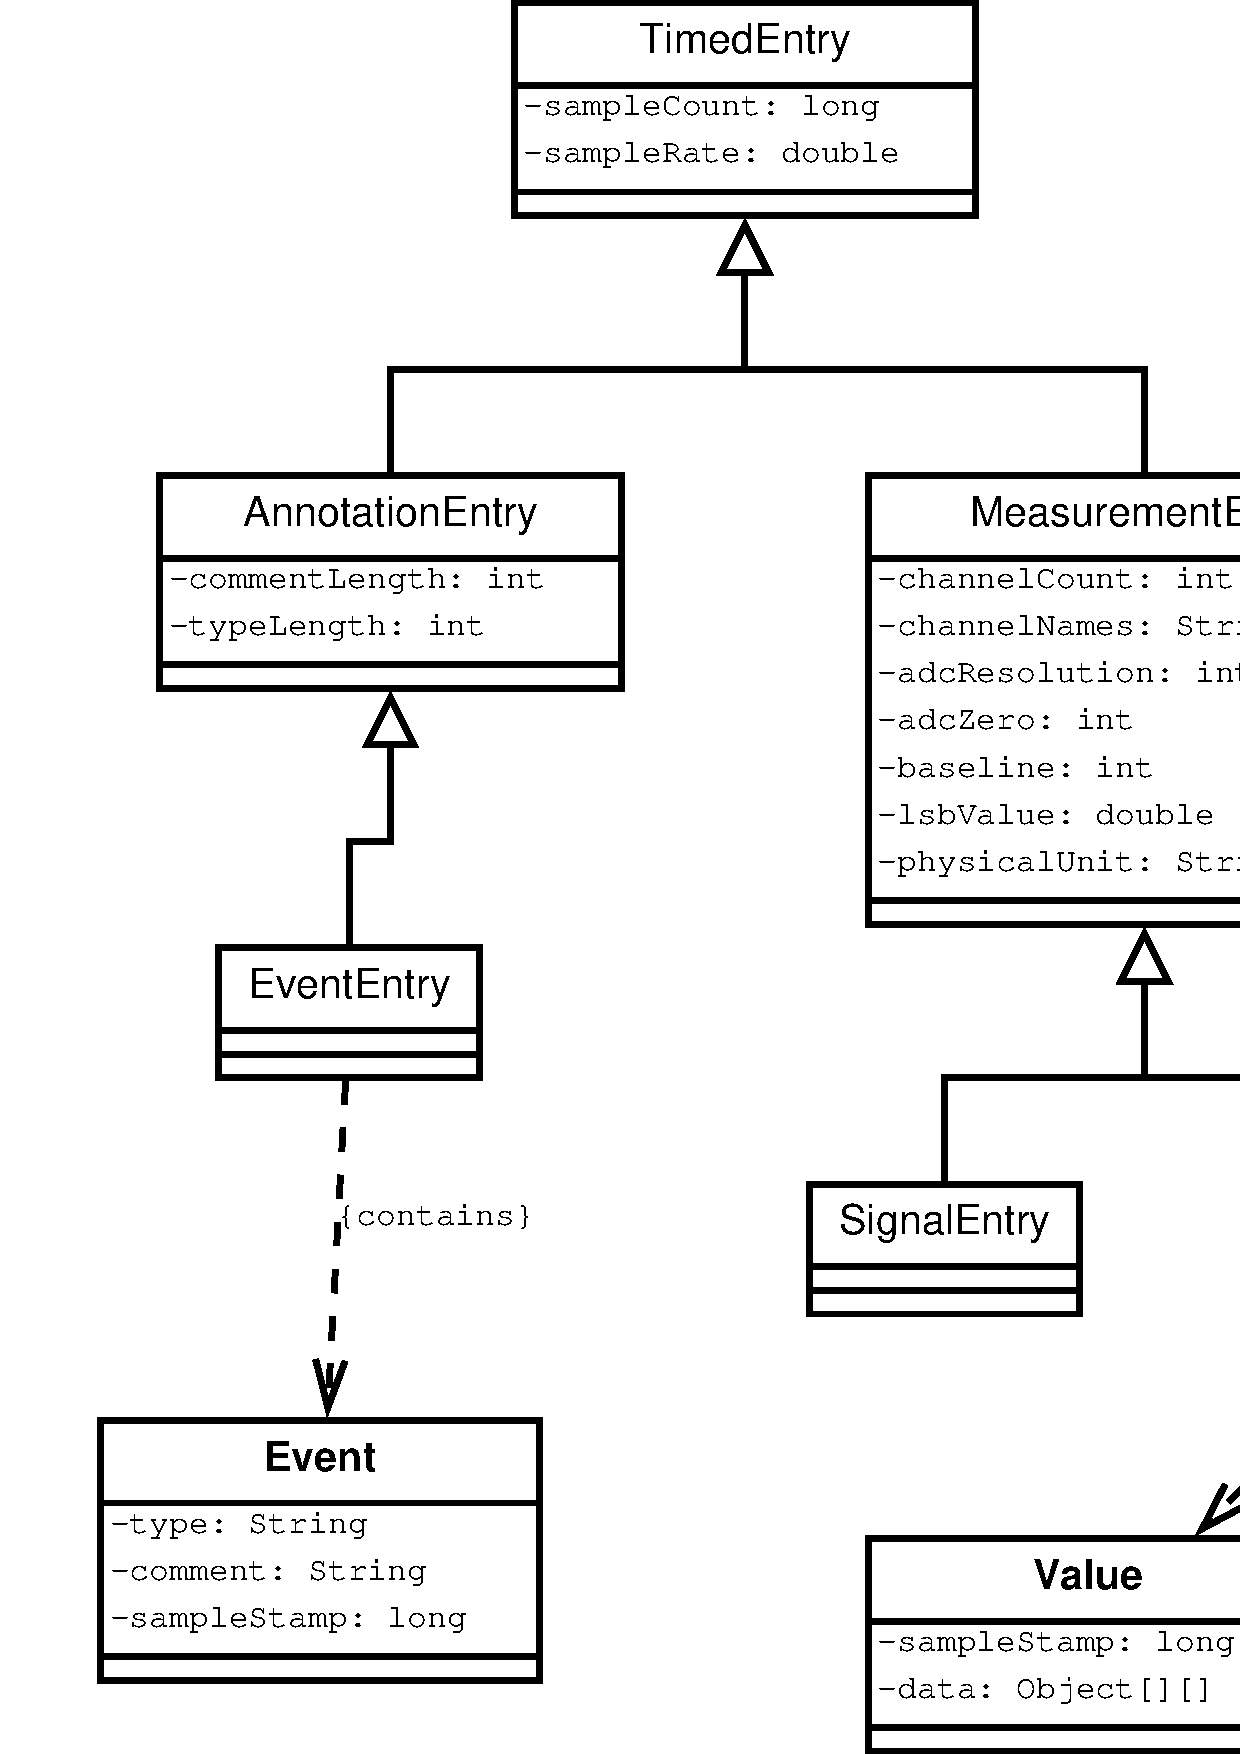
\includegraphics[width=\textwidth]{bilder/unisens_interface.png}
\caption{Klassen\"ubersicht der von Unisens definierten Schnittstellen}
\label{pic:unisens_interface}
\end{figure}
Wenn man schon vorhandene Unisensdatens\"atze benutzen m\"ochte reicht es aus, die Schnittstellendefinition zu kennen und zu nutzen.
Sollen hingegen konkret Objekte erstellt werden, muss auf die Basisimplementierung zur\"uckgegriffen werden.
Eine \"Ubersicht der Klassenstruktur und der von au\ss en ersichtlichen Attribute ist in Abbildung \ref{pic:unisens_interface} dargestellt.
Die unterst\"utzten Signalarten sind auch in der Klassenstruktur erkennbar:
\begin{table}[h]
\centering
\begin{tabular}{|c|c|}
	\hline Signale & \verb|SignalEntry| \\
	\hline Ereignisse & \verb|EventEntry| \\
	\hline Einzelwerte & \verb|ValuesEntry| \\
	\hline Propriet\"are Daten & \verb|CustomEntry| \\
	\hline
\end{tabular}
\caption{Signalarten und die dazugeh\"origen Klassen}
\label{tab:signal_klassen}
\end{table}

Aufgrund der Ableitung der Klassen \verb|EventEntry| und \verb|ValuesEntry| von \verb|TimedEntry| ist ersichtlich, dass die Zeitpunkte von Ereignisdaten und Einzelwertdaten werden \"uber eine virtuelle Abtastrate bestimmt werden.
Der Zeitpunkt eines jeden \emph{Event}- oder \emph{Value}-Eintrags ist als ganzzahlige Samplenummer dieser Abtastrate gespeichert.
Die Zeit eines Ereignisses, relativ zum Messbeginn, errechnet sich somit $Zeitpunkt = {Samplenummer \over Abtastrate}$.
M\"ochte man die M\"oglichkeit Ereignisse f\"ur jeden beliebigen Datenpunkt eines Datensatzes zuordnen zu k\"onnen, dann muss die virtuelle Abtastrate als das kleinste gemeinsame Vielfache aller vorhandenen Abtastraten gew\"ahlt werden.

Durch einen Fehler in der Basisimplementierung kann es vorkommen, dass beim Laden eines vorhandenen Unisensdatensatzes in dem Gruppen definiert sind eine \verb|NullPointerException| auftritt.
Insbesondere tritt dieser Fehler auf, wenn innerhalb der Headerdatei der Gruppeneintrag nicht hinter den Dateneintr\"agen steht.

Die Schnittstellendefinition des Unisensformats stellt nur Methoden zum Lesen und Anh\"angen von Datenpunkten an den Datensatz bereit.
Somit wird ein Einf\"ugen, L\"oschen oder Ver\"andern von Datenpunkten innerhalb eines Dateneintrags nicht unterst\"utzt.
Sollen diese Funktionen vorhanden sein, so muss diese Funktionalit\"at selbst implementiert werden.

%% EOF %%%%%%%%%%%%%%%%%%%%%%%%%%%%%%%%%%%%%%%%%%%%%%%%%%%%%%
